\documentclass[aspectratio=169, table]{beamer}

%\usepackage[beamertheme=./praditatheme]{Pradita}
\usepackage[utf8]{inputenc}

\usetheme{Pradita}

\subtitle{IT130204 - Information System \&\\Technology Architecture}

\title{Session-03:\LARGE{\\TOGAF Framework and \\ Its Components}
}
\date[Serial]{\scriptsize {PRU/SPMI/FR-BM-18/0222}}
\author[Pradita]{\vspace{10pt}\small{\textbf{Alfa Yohannis}}}

\begin{document}
	
	\frame{\titlepage}
	
	\begin{frame}
		\frametitle{What is the TOGAF Framework?}
		% \framesubtitle{\hspace{1cm}}
		\begin{itemize}
			\item TOGAF is a framework for enterprise architecture development.
			\item Developed by The Open Group, an IT industry consortium.
			\item Consists of methods and tools to assist in the design, implementation, and management of enterprise architecture.
			\item TOGAF focuses on architecture lifecycle management.
			\item Uses a repeatable and iterative life cycle approach.
		\end{itemize}
	\end{frame}
	
	\begin{frame}
		\frametitle{Architecture Domain}
		% \framesubtitle{\hspace{1cm}}
		\vspace{20pt}
		\begin{itemize}
			\item \textbf{Business Architecture}. Business strategy, governance, organisation and key business processes.
			
			\item \textbf{Data Architecture}. Organisational logical and physical data structures
			asset and resource data management.
			
			\item \textbf{Application Architecture}. A blueprint for the individual application systems that will be deployed, their interactions, and their relationships to the organization's core business processes.
			
			\item \textbf{Technology Architecture}. Software and hardware capabilities required to support the deployment of business, data, and service applications. This includes IT infrastructure, middleware, networking, communications, processing, and standards.
		\end{itemize}
	\end{frame}
	
	{
		\setbeamertemplate{frametitle}{}
		\setbeamertemplate{navigation symbols}{}
		\setbeamertemplate{footline}{}
		\begin{frame}
			\frametitle{TOGAF Framework}
			\framesubtitle{\hspace{1cm}}
			\begin{center}
				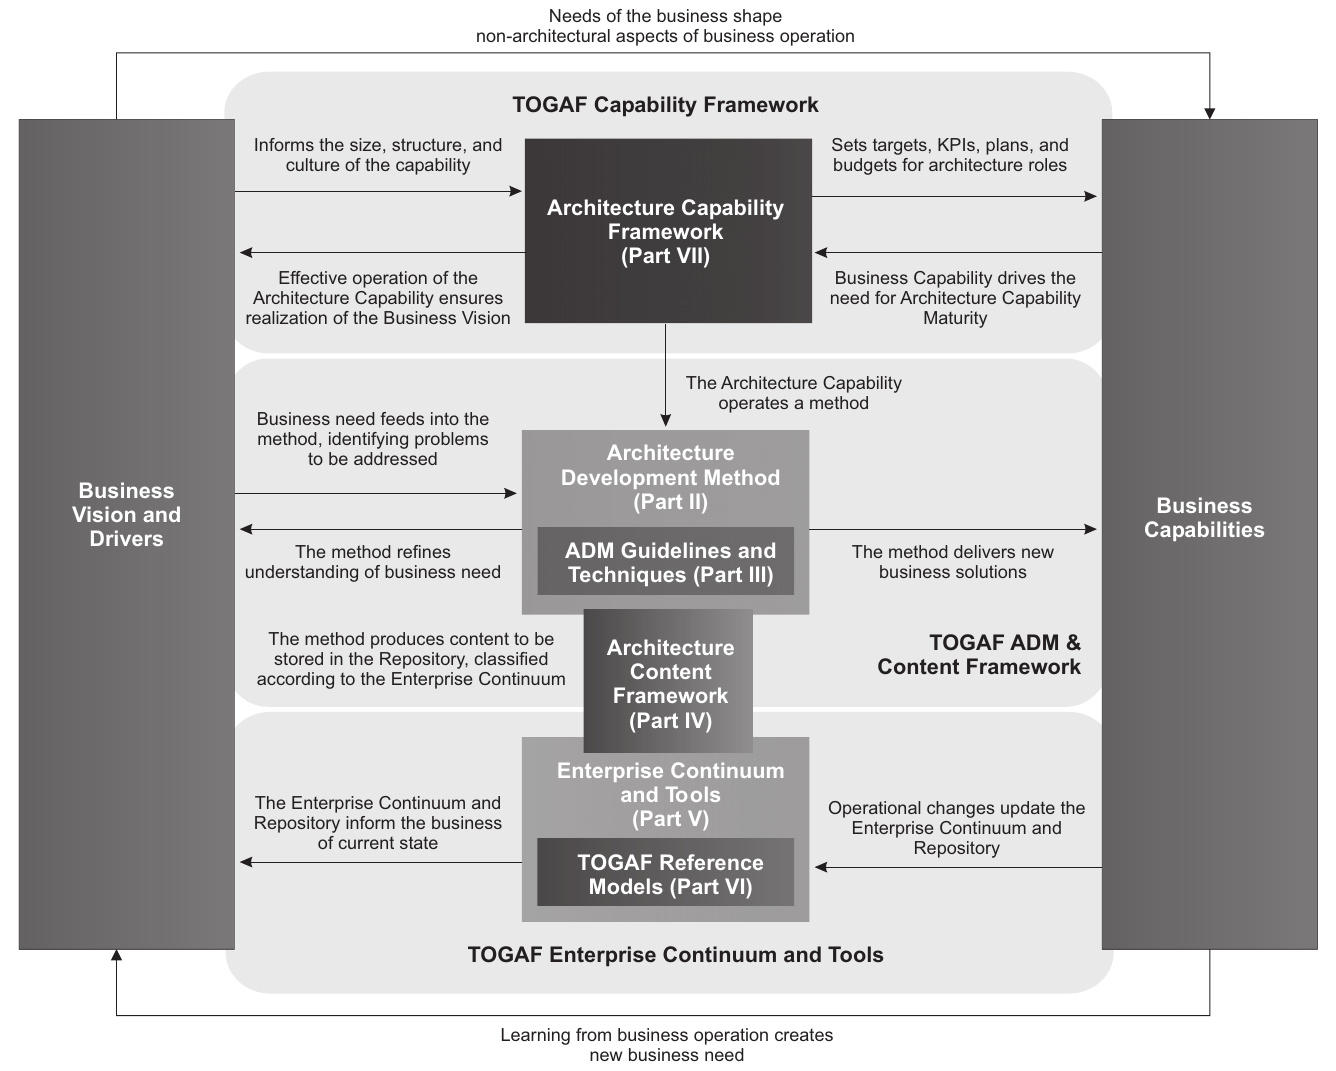
\includegraphics[width=.78\textwidth]{../figures/togaf}
			\end{center}
		\end{frame}
	}
	
	\begin{frame}
		\frametitle{TOGAF components}
		\framesubtitle{\hspace{1cm}}
		\begin{itemize}
			\item Business Visions and Drivers (1)
			\item Business Capabilities (2)
			\item Architecture Capability Framework (3)
			\item Architecture Development Method (4)
			\item ADM Guidelines and Techniques (5)
		\end{itemize}
	\end{frame}
	
	\begin{frame}
		\frametitle{TOGAF components (2)}
		\framesubtitle{\hspace{1cm}}
		\begin{itemize}
			
			\item Architecture Governance Framework 
			\item Architecture Content Framework (6)
			\item Deliverables, Artifacts, and Building Blocks
			\item Enterprise Continuum and Tools (7) 
			\item Architecture Repository
			\item TOGAF Reference Models (8)
		\end{itemize}
	\end{frame}
	
	\begin{frame}
		\frametitle{Vision and Business Drivers}
		% \framesubtitle{\hspace{1cm}}
		\begin{itemize}
			\item \textbf{\textit{What are the motivations?}}
			\item A business vision is a view of an organization's goals and future.
			\item Business drivers are factors that drive change in an organization.
			\item TOGAF uses business vision and drivers to help define enterprise architecture.
			\item The business vision and drivers are developed during the Preliminary and Architecture Vision phases of ADM.
			\item In TOGAF, business drivers can include factors such as technological changes, market changes, or regulatory changes.
		\end{itemize}
	\end{frame}
	
	\begin{frame}
		\frametitle{Business Capabilities}
		% \framesubtitle{\hspace{1cm}}
		\begin{itemize}
			\item \textbf{\textit{What are the capabilities we want to have?}}
			\item Business capabilities are the combination of people, processes, and technology that enable an organization to achieve its goals.
			\item TOGAF views business capabilities as an integral part of the enterprise architecture.
			\item A good understanding of business capabilities can help in the design and implementation of effective architectures.
			\item Business capabilities are identified and defined during the ADM process.
			\item They are then used to assist in architecture design and implementation.
		\end{itemize}
	\end{frame}
	
	
	\begin{frame}
		\frametitle{\LARGE{TOGAF Architecture Capability Framework}}
		%        \framesubtitle{\hspace{1cm}}
		\vspace{20pt}
		\begin{itemize}
			\item TOGAF 9 provides an Architecture Capability Framework which is a collection of reference materials and guidelines for building architecture functions
			or capabilities in the organization.
			\item Consists of seven components: creating architecture capabilities, architecture board, architecture compliance, architecture contracts, architecture governance, architecture maturity models, and architecture skills frameworks.
			\item Each component covers a set of capabilities necessary to produce an effective enterprise architecture.
			\item Using the Capability Framework, organizations can identify and close gaps in their capabilities.
		\end{itemize}
	\end{frame}
	
	{
		\setbeamertemplate{frametitle}{}
		\setbeamertemplate{navigation symbols}{}
		\setbeamertemplate{footline}{}
		\begin{frame}
			\frametitle{Architecture Capability Framework}
			\framesubtitle{\hspace{1cm}}
			\begin{center}
				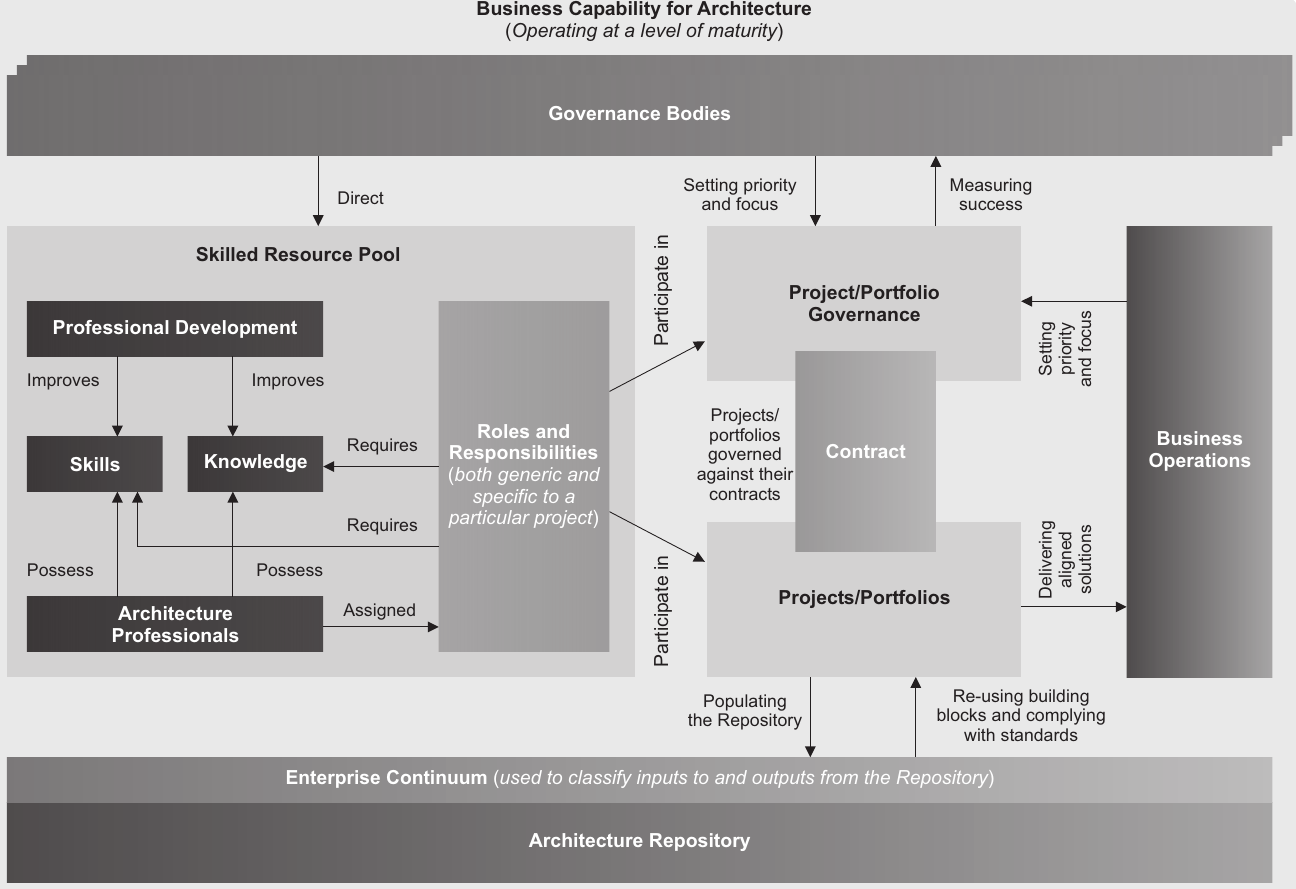
\includegraphics[width=.80\textwidth]{../figures/architecture_capability_framework}
			\end{center}
		\end{frame}
	}
	
	\begin{frame}
		\frametitle{Components of the TOGAF Architecture Capability Framework}
		\framesubtitle{\hspace{1cm}}
		\begin{enumerate}
			\item \textbf{\textit{What do we need to have in order to gain those capabilities?}}
			\item \textbf{Creating a Capability Architecture}. Setting up the necessary structures, processes, and roles to support the organization’s architecture practice (incl. scope, stakeholders, governance).
			\item \textbf{Architecture Board}. Overseer for the establishment and operation of the company's Architecture Council.
			\item \textbf{Architecture Compliance}.  Ensures that the organization’s architecture complies with relevant standards, policies, and regulations.
			\item \textbf{Architecture Contract}. Agreements that define define the scope, objectives, and deliverables.
		\end{enumerate}
	\end{frame}
	
	\begin{frame}
		\frametitle{Contents of the TOGAF Architecture Capability Framework (2)}
		\framesubtitle{\hspace{1cm}}
		\begin{enumerate}
			\setcounter{enumi}{4}
			\item \textbf{Architecture Governance}.  Ensures that the organisation’s architecture is aligned with business strategy and goals.
			\item \textbf{Architecture Maturity Model}. Help organisations assess the maturity of their architecture practice and identify areas for improvement.
			\item \textbf{Architecture Skills Framework}. A set of roles, skills, and experience norms for staff performing enterprise architecture work.
		\end{enumerate}
	\end{frame}
	
	
	\begin{frame}
		\frametitle{Architecture Development Method (ADM)}
		\begin{itemize}
			\item \textbf{\textit{How or what actions should we do to gain those capabilities?}}
			\item ADM is the process recommended by TOGAF for developing enterprise architecture.
			\item Involves a series of organized phases that help in the design, planning, implementation, and management of enterprise architecture.
			\item These phases include Architecture Vision, Business Design, Information Design, Technology Design, to Implementation.
			\item ADM helps organizations manage the entire lifecycle of an enterprise architecture.
			\item ADM also provides guidelines and techniques for each phase of the development process.
		\end{itemize}
	\end{frame}
	
	{
		\setbeamertemplate{frametitle}{}
		\setbeamertemplate{navigation symbols}{}
		\setbeamertemplate{footline}{}
		\begin{frame}
			\frametitle{Architecture Development Method}
			\framesubtitle{\hspace{1cm}}
			\begin{center}
				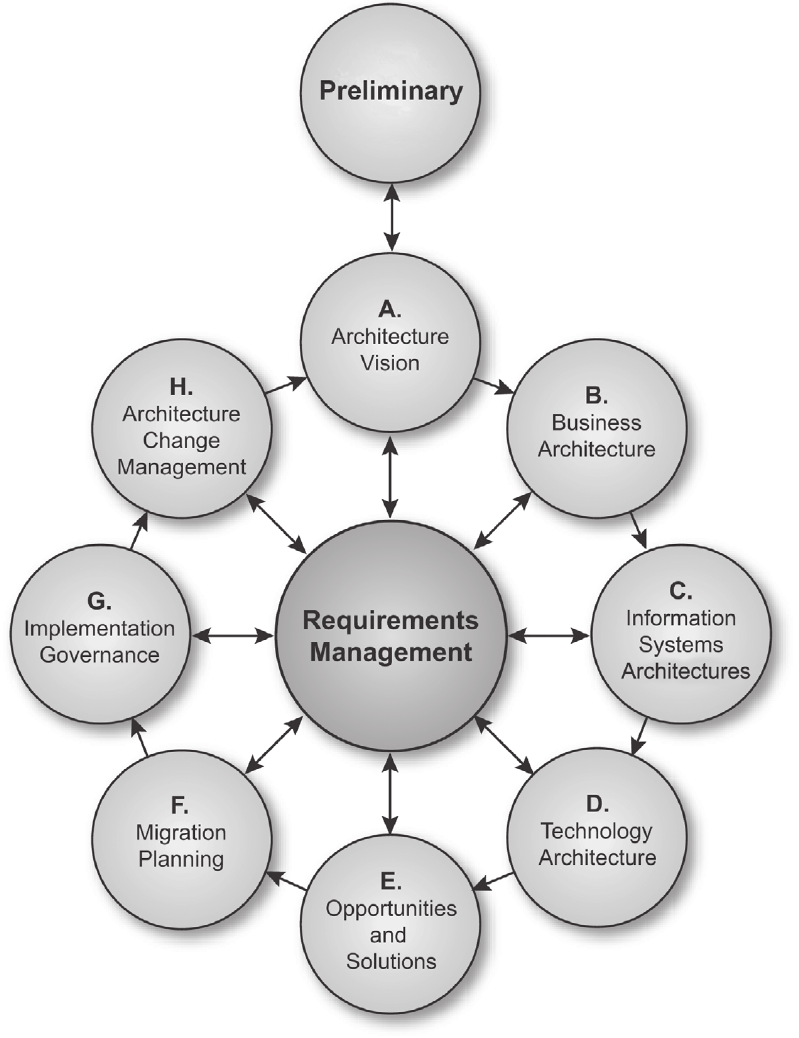
\includegraphics[width=.43\textwidth]{../figures/architecture_development_method}
			\end{center}
		\end{frame}
	}
	
	\begin{frame}
		\frametitle{ADM Guidelines and Techniques}
		% \framesubtitle{\hspace{1cm}}
		\vspace{15pt}
		\begin{itemize}
			\item \textbf{\textit{Are there any guidances and techniques to do the actions?}}
			\item TOGAF provides a set of guidelines and techniques to assist in the implementation of ADM.
			\item This guidance helps organizations adapt ADM to their own needs and context.
			\item Some commonly used techniques include principles analysis, stakeholder analysis, gap analysis, business scenarios, migration plans, interoperability, risk management, capability plans.
			\item These guidelines and techniques ensure that the ADM process remains focused, efficient, and effective.
			\item Guidelines also help ensure that the resulting architecture aligns with business goals and objectives.
			\item \url{https://pubs.opengroup.org/architecture/togaf92-doc/m/pt3.html}
		\end{itemize}
	\end{frame}
	
	\begin{frame}
		\frametitle{Architecture Governance Framework}
		\begin{itemize}
			\item \textbf{\textit{How to control and ensure that we are on the right track?}}
			\item Architecture governance is the practice of managing and controlling an enterprise's architecture.
			\item In TOGAF, the architecture governance framework provides a structure for these practices.
			\item This framework includes aspects such as organizational structure, roles and responsibilities, processes, and communication methods.
			%			\item Architecture governance also involves creating and maintaining artifacts such as architecture principles, architecture models, and architecture roadmaps.
			\item The primary goal is to ensure that all projects remain aligned with the enterprise architecture and overall business strategy.
		\end{itemize}
	\end{frame}
	
	\begin{frame}
		\frametitle{Architecture Content Framework}
		% \framesubtitle{\hspace{1cm}}
		\begin{itemize}
			\item \textbf{\textit{What are the required elements to bring those capabilities to life?}}
			\item The Architecture Content Framework defines the types of architecture content required to cover the entire business domain.
			\item It guides the process of artifact identification, organization, and development.
			\item The Architecture Content Framework consists of three main components: Deliverables, Artifacts, and Building Blocks.
		\end{itemize}
	\end{frame}
	
	
	
	\begin{frame}
		\frametitle{Deliverables, Artifacts, and Building Blocks}
		\framesubtitle{in Architecture Content Framework}
		\begin{itemize}
			\item \textbf{Deliverables} are the results of architecture work provided to stakeholders. For example, Technology Architecture Document, Architecture Vision Document, Migration Plan.
			\item \textbf{Artifacts} are parts of Deliverables that describe the architecture in varying levels of detail. For example, Lists/Catalogues of software, Matrix of Applications, Data Diagrams, Network Diagrams. 
			\item \textbf{Building Blocks} are groups of physical, logical, or conceptual components of a business or IT system for specific purposes. For example, data storage component, security model. They can be the concepts/designs (Architecture Building Blocks) or the actual products, technologies, or systems (Solution Building Blocks).
		\end{itemize}
	\end{frame}
	
	{
		\setbeamertemplate{frametitle}{}
		\setbeamertemplate{navigation symbols}{}
		\setbeamertemplate{footline}{}
		\begin{frame}
			\frametitle{Architecture Deliverables}
			\framesubtitle{\hspace{1cm}}
			\begin{center}
				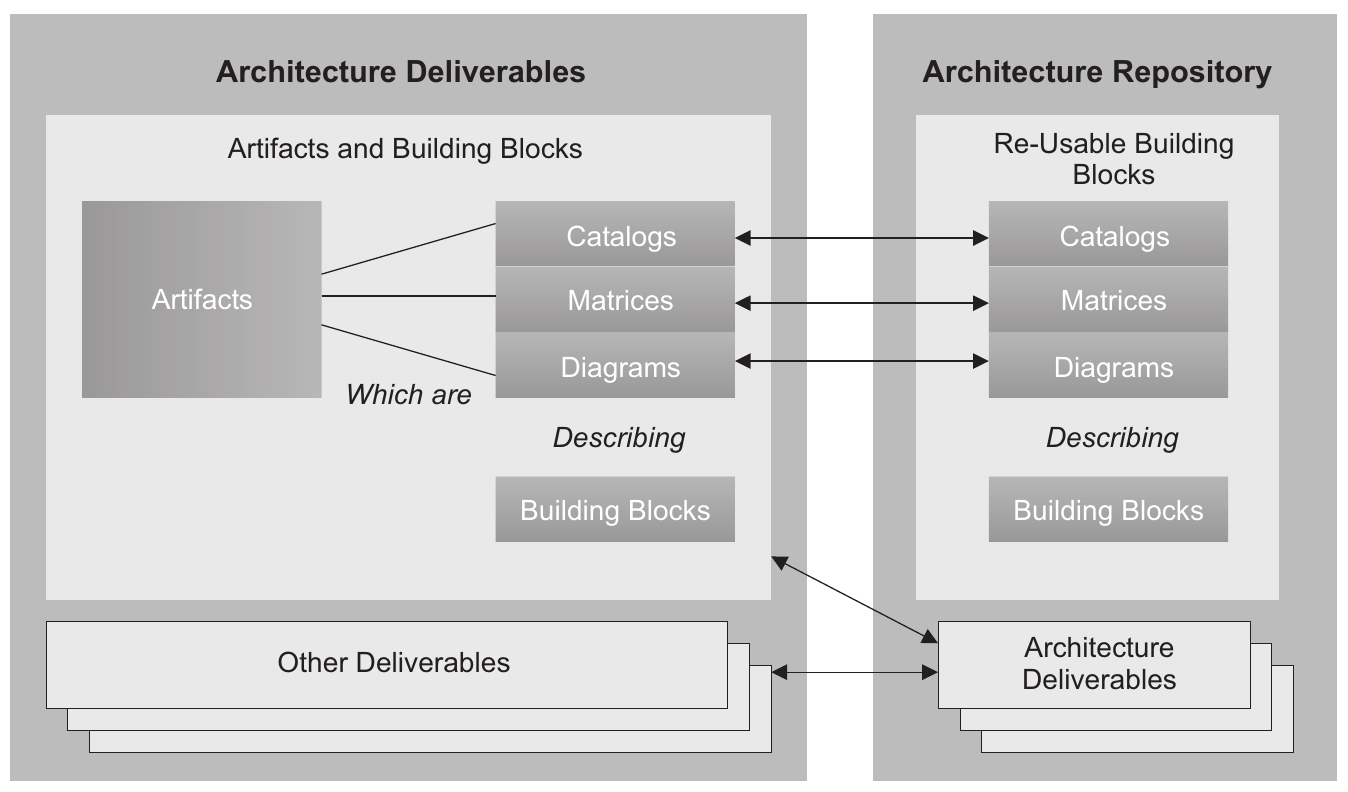
\includegraphics[width=.95\textwidth]{../figures/architecture_deliverables}
			\end{center}
		\end{frame}
	}
	
	
	
	\begin{frame}
		\frametitle{Enterprise Continuum and Tools}
		% \framesubtitle{\hspace{1cm}}
		\vspace{20pt}
		\begin{itemize}
			\item \textbf{\textit{What are the available solutions, standards, or best practices, both externally and internally, that we could make use of?}}
			\item The Enterprise Continuum is a general-to-specific perspective or guide that provides a context for understanding and managing architecture artifacts.
			\item This helps organizations identify and utilize relevant artifacts based on their needs.
			\item Enterprise Tools are the tools and techniques used to support the creation, management, and use of architectures.
			\item Examples of these tools include modeling software, project management tools, and documentation tools.
			\item This tool supports organizations in implementing and managing their enterprise architecture.
		\end{itemize}
	\end{frame}
	
	{
		\setbeamertemplate{frametitle}{}
		\setbeamertemplate{navigation symbols}{}
		\setbeamertemplate{footline}{}
		\begin{frame}
			\frametitle{Architecture Continuum}
			\framesubtitle{\hspace{1cm}}
			\begin{center}
				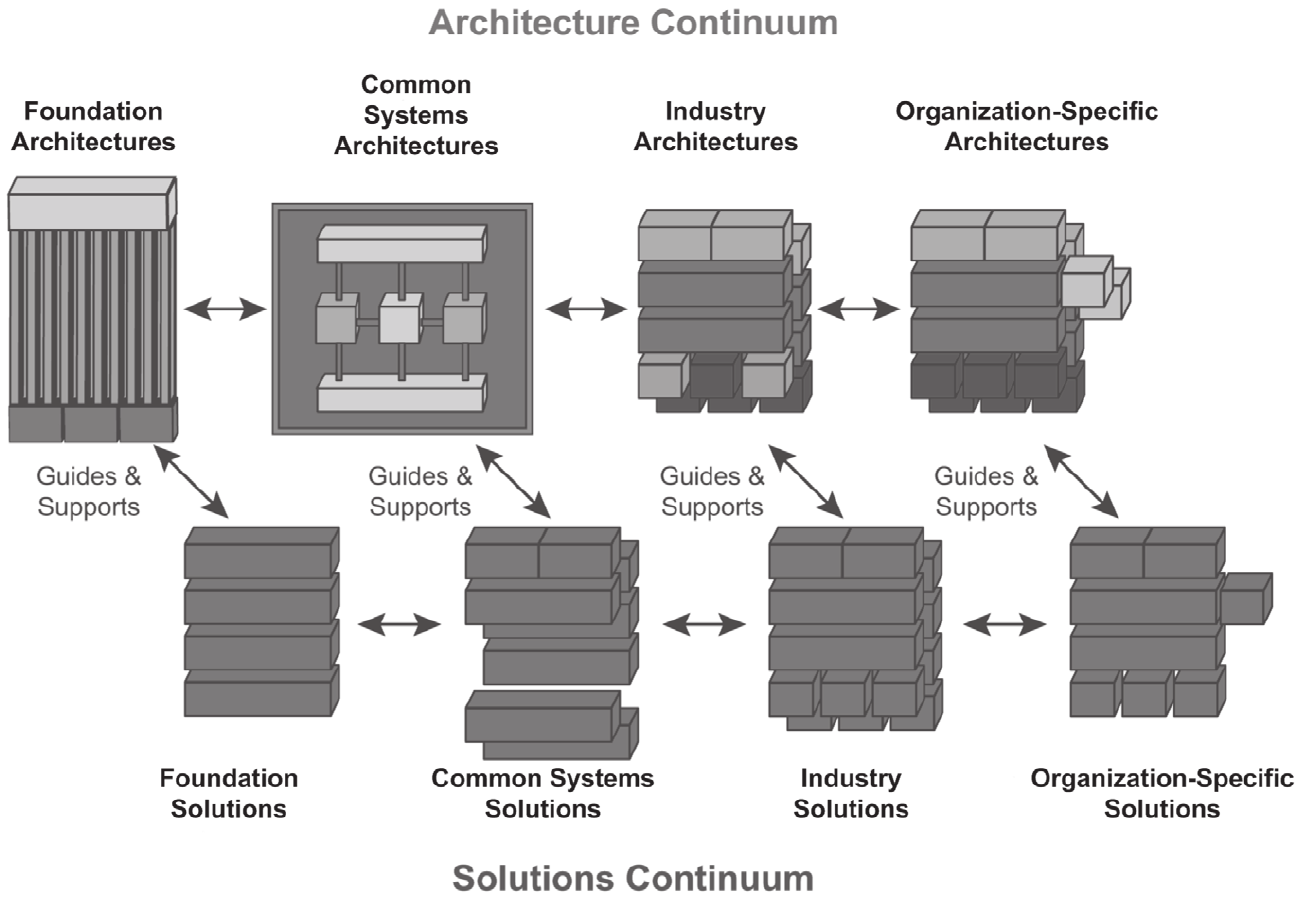
\includegraphics[width=.80\textwidth]{../figures/enterprise_continuum}
			\end{center}
		\end{frame}
	}
	
	\begin{frame}
		\frametitle{Architecture Continuum in TOGAF}
		\vspace{10pt}
		\begin{itemize}
			\item \textbf{Foundation Architecture}: 
			\begin{itemize}
				\item Example: Generic cloud computing architecture defining IaaS, PaaS, and SaaS components.
			\end{itemize}
			\item \textbf{Common System Architecture}: 
			\begin{itemize}
				\item Example: ERP system architecture integrating finance, HR, and supply chain functions.
			\end{itemize}
			\item \textbf{Industry-Specific Architecture}: 
			\begin{itemize}
				\item Example: Healthcare information system architecture including EHR and patient management, compliant with HIPAA.
			\end{itemize}
			\item \textbf{Organization-Specific Architecture}: 
			\begin{itemize}
				\item Example: Custom architecture for a specific hospital.
			\end{itemize}
		\end{itemize}
	\end{frame}
	
	
	\begin{frame}
		\frametitle{Architecture Repository in TOGAF}
		% \framesubtitle{\hspace{1cm}}
		\vspace{20pt}
		\begin{itemize}
			\item \textbf{\textit{Essentially, it is a storage or library of all outputs, solutions, and information gathered in the previous or ongoing enterprise architecture activities.}}
			\item The Architecture Repository is an organized repository for all artifacts produced by an architect during the ADM lifecycle.
			\item This repository helps in the storage, management, and reuse of architecture information.
			%			\item The architecture landscape in a repository involves three levels: strategic architecture, segment architecture, and capability architecture.
			%			\item This repository also supports the management and monitoring of Architecture Contracts.
			\item This repository makes it easy to manage artifacts and deliverables in a multi-project environment.
		\end{itemize}
	\end{frame}
	
	
	
	{
		\setbeamertemplate{frametitle}{}
		\setbeamertemplate{navigation symbols}{}
		\setbeamertemplate{footline}{}
		\begin{frame}
			\frametitle{Architecture Repository}
			\framesubtitle{\hspace{1cm}}
			\begin{center}
				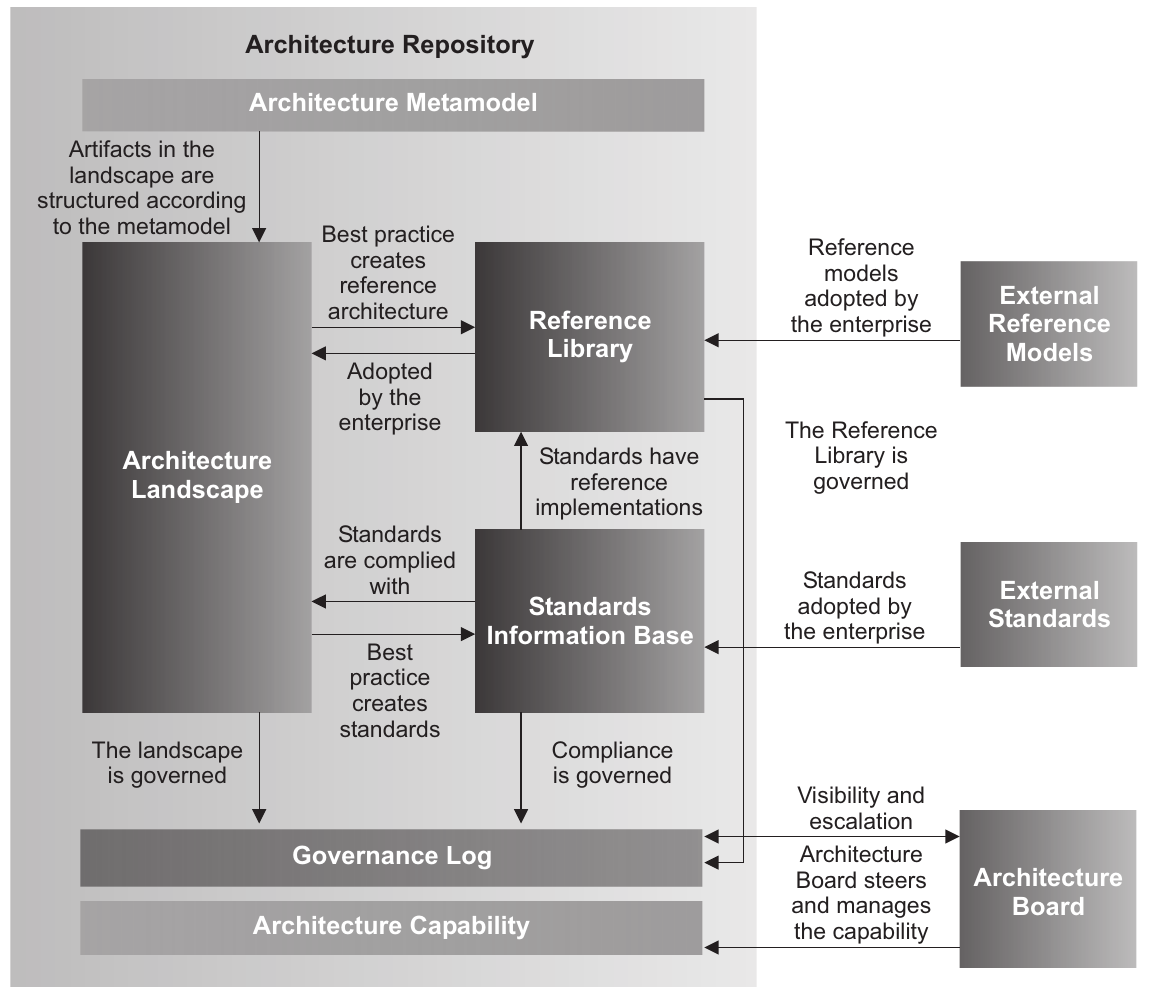
\includegraphics[width=.65\textwidth]{../figures/architecture_repository}
			\end{center}
		\end{frame}
	}
	
	\begin{frame}
		\frametitle{Architecture Repository Components}
		\vspace{20pt}
		\begin{itemize}
			\item \textbf{Architecture Metamodel}: Framework or description defining the structure and relationships of architecture elements. 
			\item \textbf{Architecture Landscape}: It contains the artifacts structured by the architecture metamodel, sometimes presented in diagrams.			
			\item \textbf{Reference Library}: It contains reference architectures -- architectures produced through best practices. E.g., architectural patterns, business process patterns.
			\item \textbf{Standards Information Base}: Repository standards and guidelines. E.g., data storage standards, ISO standards.
			\item \textbf{Governance Log}: Records of governance decisions and activities. E.g., minutes of board meetings.
			\item \textbf{Architecture Capability}: The repo of the organization’s capabilities. E.g., e-commerce initiative, secure parking, customers profiling. 
		\end{itemize}
	\end{frame}
	
	\begin{frame}
		\frametitle{TOGAF Reference Model}
		% \framesubtitle{\hspace{1cm}}
		\begin{itemize}
			\item \textbf{\textit{Where should I begin when building a solution?}}
			\item The TOGAF Reference Model is a framework that provides a useful starting point for organizations seeking help with their architecture initiatives.
			\item This provides a basic model that can be used as a basis for developing more specific and detailed architectures.
			\item TOGAF Reference Models include the Technical Reference Model (TRM) and the Integrated Information Infrastructure Reference Model (III-RM).
			
		\end{itemize}
	\end{frame}
	
	\begin{frame}
		\frametitle{TOGAF Reference Model (2)}
		% \framesubtitle{\hspace{1cm}}
		\begin{itemize}
			\item TRM provides a common model and taxonomy for the technologies that support business applications, such as operating systems, hardware, and networks.
			\item Integrated Information Infrastructure (III-RM) provides a model for architecture and components that enable greater application portability, interoperability, and reuse.
		\end{itemize}
	\end{frame}
	
	{
		\setbeamertemplate{frametitle}{}
		\setbeamertemplate{navigation symbols}{}
		\setbeamertemplate{footline}{}
		\begin{frame}
			\frametitle{Technical Reference Model}
			\framesubtitle{\hspace{1cm}}
			\begin{center}
				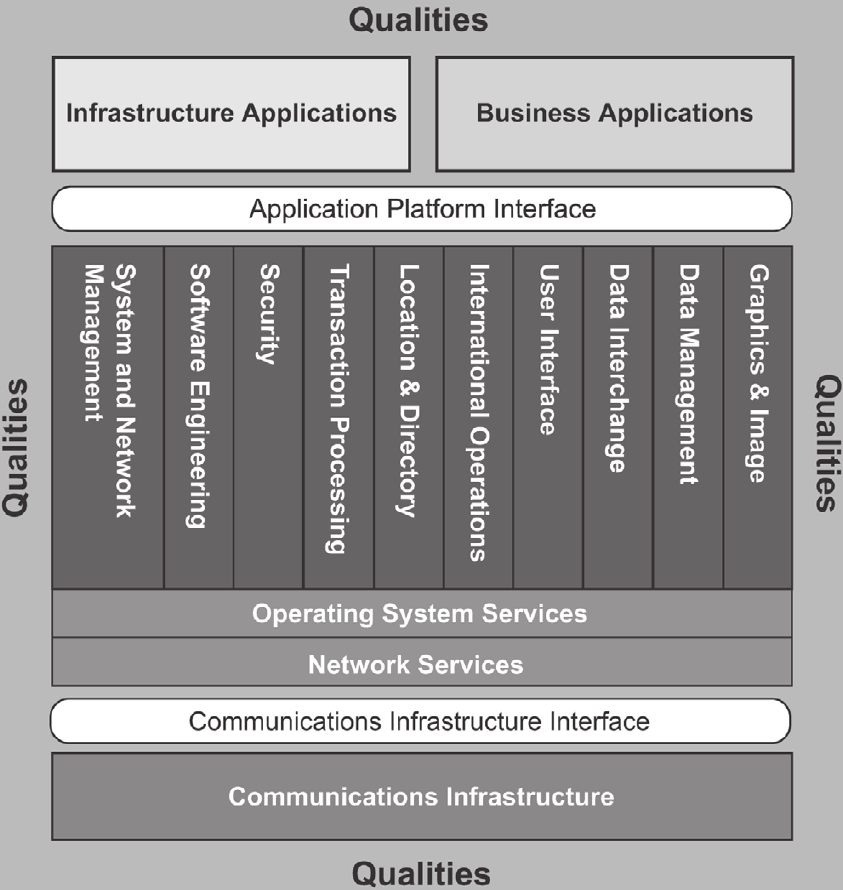
\includegraphics[width=.53\textwidth]{../figures/detailed_technical_reference_model}
			\end{center}
		\end{frame}
	}
	
	{
		\setbeamertemplate{frametitle}{}
		\setbeamertemplate{navigation symbols}{}
		\setbeamertemplate{footline}{}
		\begin{frame}
			\frametitle{Integrated Information Infrastructure Reference Model}
			\framesubtitle{\hspace{1cm}}
			\begin{center}
				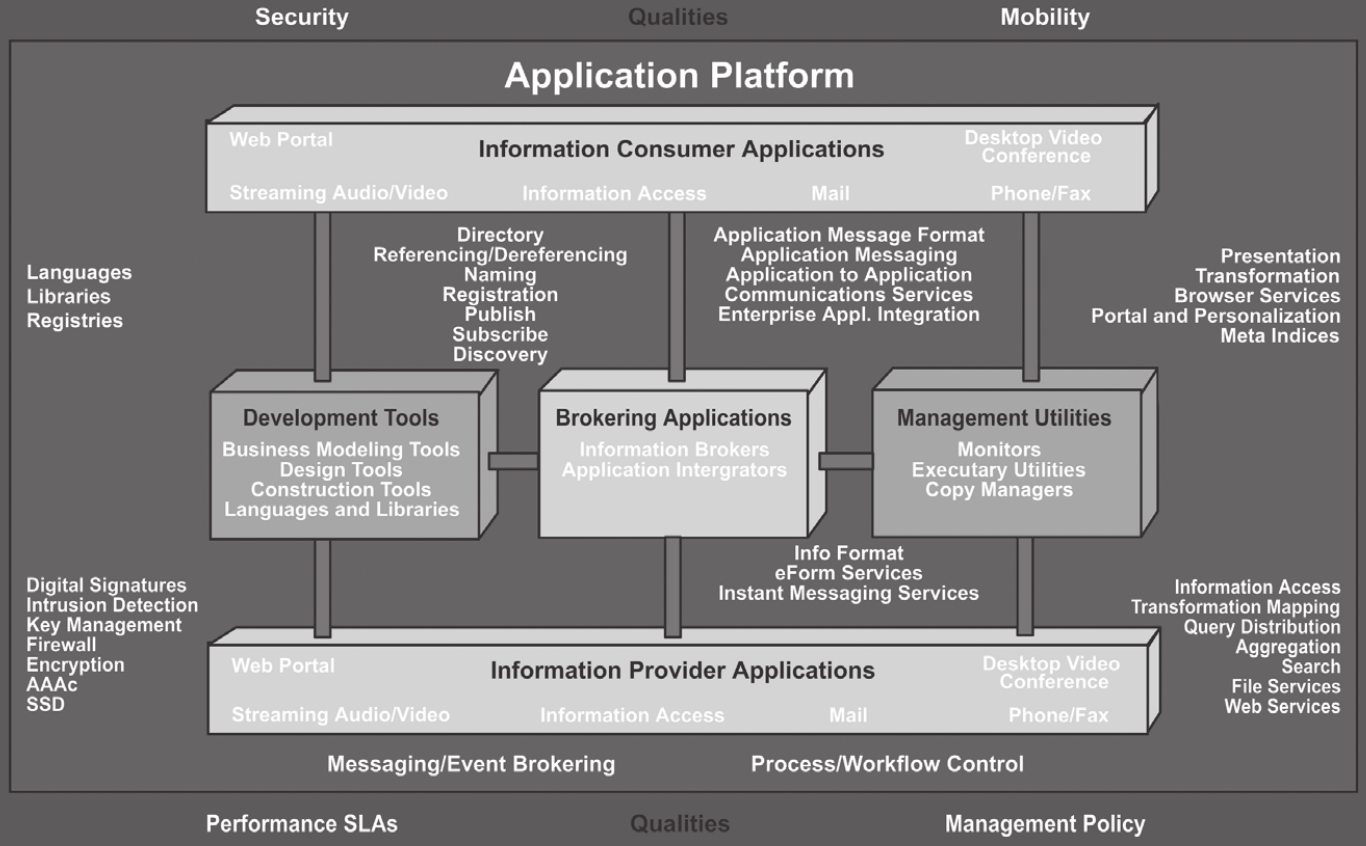
\includegraphics[width=.90\textwidth]{../figures/integrated_information_infrastructure_reference_model}
			\end{center}
		\end{frame}
	}
	
	\begin{frame}
		\frametitle{Summary}
		% \framesubtitle{\hspace{1cm}}
		\begin{itemize}
			\item TOGAF is a comprehensive enterprise architecture framework that helps organizations design, plan, implement, and manage their information architecture.
			\item TOGAF involves various aspects such as business vision and drivers, business capabilities, capability frameworks, architecture development methods, and others.
			\item In TOGAF, artifacts, deliverables, and building blocks are used to assist in the architecture development process.
		\end{itemize}
	\end{frame}
	
	\begin{frame}
		\frametitle{Summary (2)}
		% \framesubtitle{\hspace{1cm}}
		\begin{itemize}
			\item The enterprise continuum and tools in TOGAF help organizations understand and utilize this framework effectively.
			\item The TOGAF Architecture Repository and Reference Model is an important knowledge reference component to support the ADM process.
		\end{itemize}
	\end{frame}
	
	
\end{document}